\section{Residual \B background subtraction} \label{sec:post_fit}

The resulting peaking $B$ yields include contributions from \BtoXsgamma events and other correctly-tagged \BB processes, which are considered background. Due to the high-purity of the tagged sample, background contamination is low at high-\EB, but grows sharply with decreasing \EB. 

To remove this background, the PDFs defined in \Cref{sec:fitting_procedure} are used to fit simulated \BB samples in which \BtoXsgamma events are removed. This procedure extracts yields of peaking nonsignal events in every \EB bin. The background predictions are scaled for luminosity, and corrected based on FEI calibration factors \cite{Belle-II:2020fst}, \g~detection-efficiency \cite{gamma_eff}, and \piz~efficiency. Branching fractions used in simulation for the background modes are matched to the most recent known values. The \mbox{$1.4<\EB<1.8\gev$} region, where signal purity is low, is used for validating the background subtraction. Event yields observed in data after subtraction are compared with expectations from background-only simulation. An 8.7\% difference is observed, which is assigned as a uniform correction factor for background normalisation across bins. The background expectations from simulation and observed yields in data are shown in \Cref{fig:background_vs_data}.
 
 \begin{figure}[htbp!]
     \centering
     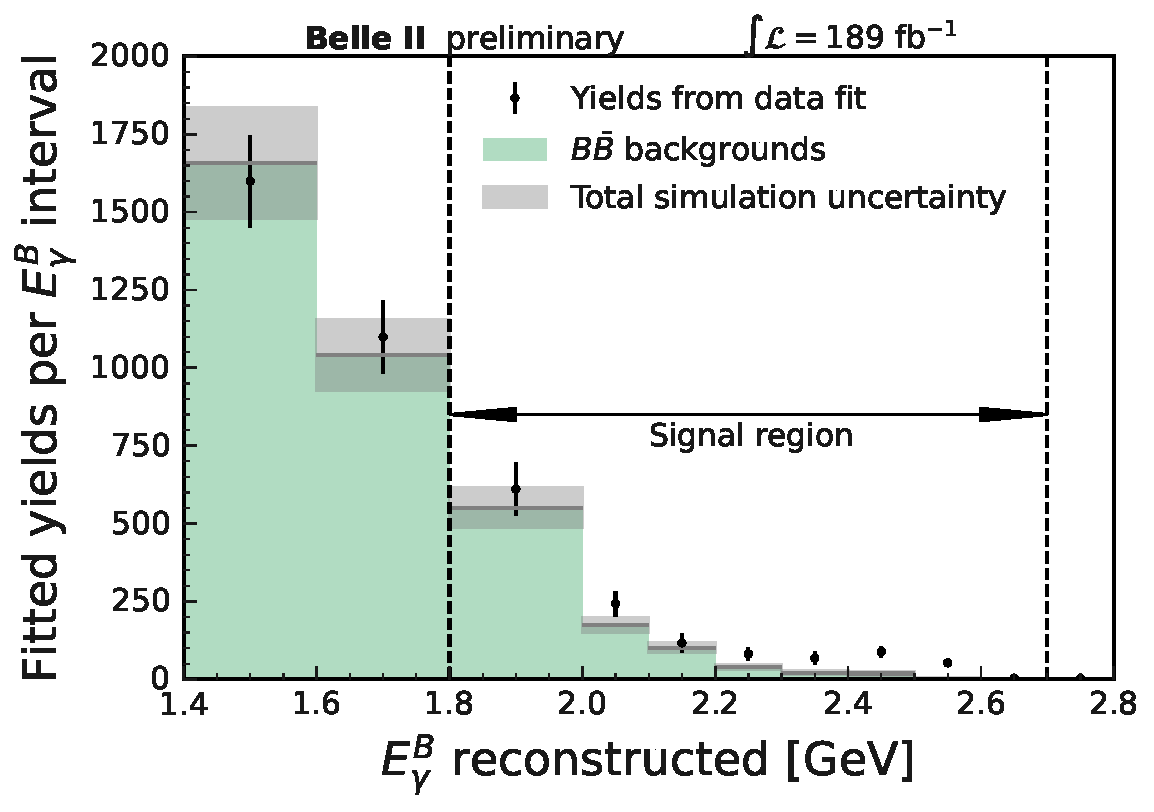
\includegraphics[width=0.5\textwidth]{results/plots/background_vs_data.pdf}
     \caption{Yield of \BB events as a function of photon energy in the signal \B meson rest frame. The data points correspond to the yields from the fits on the data \Mbc distributions. The histogram shows the luminosity-scaled yields from the background-only simulated sample. The gray bands correspond to systematic uncertainties on the \BB background prediction. The excess of events in data with respect to the \BB background is the $\B\ra X_{s+d}\g$ contribution. }
     \label{fig:background_vs_data}
 \end{figure}

\section{Unfolding}\label{sec:unfolding}

The measured \BtoXsgamma spectrum needs to be corrected (unfolded) for smearing effects. The unfolding is achieved by using bin-by-bin multiplicative factors based on the hybrid model. These factors are defined as the ratios between the expected number of events of the generated spectrum and the expected number of corresponding events of the reconstructed spectrum within an \EB interval. The measured \BtoXsgamma yields are multiplied by the unfolding factors (see \Cref{sec:results}). The bulk of the unfolding factors do not exceed 10-20\% range, and only the edge bins have 30-60\% corrections.

\section{Uncertainties}\label{sec:uncertainties}

Multiple sources of systematic uncertainty are considered and are grouped as follows: uncertainties due to assumptions in the fit; uncertainties affecting the signal efficiency estimation; data-MC normalisation in the background estimation; and other sources, such as unfolding procedure, branching fraction normalization and the subtraction of $\B\ra X_d \gamma$ component. The statistical uncertainties of the yields extracted from the fit on data are dominant.

\subsection{Uncertainties due to assumptions in the fit}\label{sec:data_uncertainty}

To account for assumptions on the values of model parameters, we repeat the fits by varying the Chebyshev polynomial coefficients by their one-standard-deviation uncertainties, and take the maximum shift in signal yield as the uncertainty. We account for a known data-simulation mismodelling of the \Mbc endpoint due to non-simulated run-dependant variations of the collision energy. The signal yields observed in data using alternative models of background shapes with various \Mbc endpoints are compared. The maximum variation with respect to the central result is taken as uncertainty.


\subsection{Signal efficiency uncertainties}\label{sec:signal_uncertainty}

The signal efficiency is calculated using the simulated hybrid-model signal sample. The values are corrected using FEI simulation-to-data calibration factors, $\mathcal{C}_{\Bz/\Bp}$ \cite{Belle-II:2020fst}, as well as acceptance corrections from the \piz veto and \g efficiency. The corresponding uncertainties related to these factors are propagated as systematic uncertainties. The signal efficiency is validated in the high-purity $\EB \in [2.5, 2.6]~\gev$ region, and the observed difference assigned as an uncertainty. 

\subsection{Background uncertainties}\label{sec:background_uncertainty}

The uncertainties associated with the limited size of the simulated samples used in the \Mbc fits are propagated to the final results. Similarly to the signal efficiency, the background yields extracted from the fits on simulated samples are corrected using FEI calibration, \piz veto efficiency, and \g detection-efficiency correction factors. Uncertainties on the branching fractions of background decay modes are also included. The observed background-normalisation difference (see \Cref{sec:post_fit}) is assigned as a 100\% systematic uncertainty. 


\subsection{Other uncertainties}\label{sec:other_uncertainty}

To unfold the measured \EB spectrum, we evaluate the hybrid-model shape uncertainties by taking into account the uncertainty on the ratio of the known branching fractions of $\B\ra\Kstar\g$ to that of  \BtoXsgamma. The \BtoXsgamma model-parameter uncertainties, based on Ref.~\cite{simba}, are also included. The analysis does not distinguish between $X_s$ and $X_d$ final-states. The contribution from the $B\ra X_d\gamma$ component is subtracted assuming the same shape and selection efficiency as \BtoXsgamma. Under this assumption, the $\mathcal{B}(\BtoXsgamma)$ and $\mathcal{B}(\B\ra X_d\g)$ ratio equals $\left|{V_{td}}/{V_{ts}}\right|^2$. The full size of the $B\ra X_d\g$ component is assigned as an uncertainty. The uncertainty on the number of $B$ meson pairs, used as the branching-fraction normalization, is also taken into account. It is estimated by an independent study with a data-driven method in which off-resonance data are used to subtract the non-\BB contribution from the on-resonance data.

\section{Results}\label{sec:results}

The partial branching fractions in the various \EB intervals are calculated as

\begin{equation}\label{eq:branching_fraction}
    \frac{1}{\Gamma_B}\frac{d\Gamma_i}{dE_{\g}} = \frac{\mathcal{U}_i\times(N^{\mathrm{DATA}}_i - N^{\mathrm{BKG,~MC}}_i-N_i^{B\rightarrow X_d \gamma})}{\varepsilon_i \times N_B},
\end{equation}

where

\begin{itemize}
    \item $N^{\mathrm{DATA}}_i$ is the peaking-$B$ yield extracted from fitting the data distributions,
    \item $N^{\mathrm{BKG,~MC}}_i$ is the non-\BtoXsgamma peaking-$B$ yield expectation extracted from fitting simulated distributions, scaled for luminosity and corrected as discussed in \Cref{sec:post_fit},
    \item $N_i^{B\rightarrow X_d \g}$ is the number of $B\rightarrow X_d \g$ events, equal to $|{V_{td}}/{V_{ts}}|^2 \approx 4.3 \% $ \cite{Workman:2022ynf} of  $N_i^{B\rightarrow X_s \g}$, assuming the same shape and selection efficiency as \BtoXsgamma,
    \item $\varepsilon_i$ is the \BtoXsgamma selection and tagging efficiency, calculated using the simulated hybrid-model sample,
    \item $\mathcal{U}_i$ is the bin-by-bin unfolding factor calculated using the simulated hybrid-model sample,
    \item $N_B\equiv2\times(198 \pm 3)\times10^6$ is the number of \B mesons in the $189~\invfb$ data sample.
\end{itemize}

The resulting partial branching fractions are shown in \Cref{fig:partial_bfs}. The various contributions from the major sources of systematic uncertainties as functions of \EB are shown in \Cref{tab:partial_bfs}.

\begin{figure}[htbp!]
    \centering
    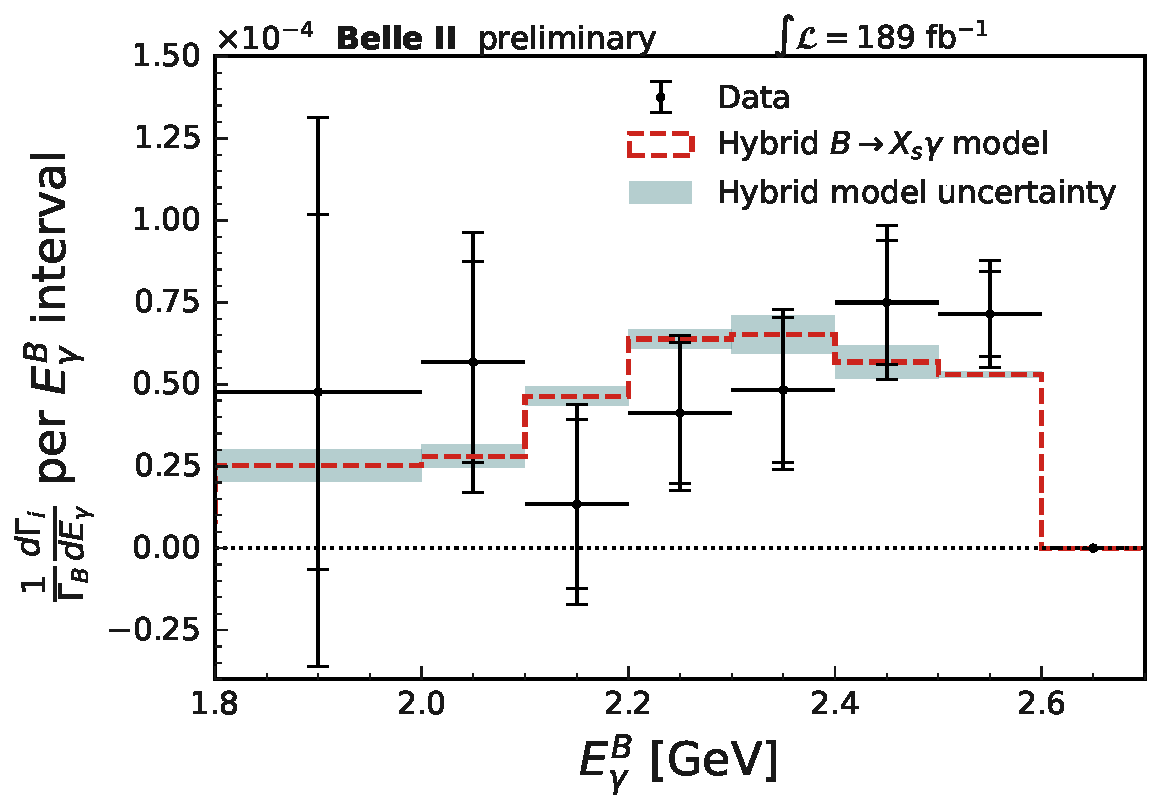
\includegraphics[width=0.5\textwidth]{results/plots/final_partial_bfs_expectation.pdf}
    \caption{Measured partial branching fractions $ (1/\Gamma_B)(d\Gamma_i/dE^B_{\g})$ as a function of \EB. The outer (inner) uncertainty bar shows the total (statistical) uncertainty. The overlaid model and uncertainty corresponds to the hybrid model.}
    \label{fig:partial_bfs}
\end{figure}

\begin{table}[htbp!]
    \centering
    \caption{Results of the partial branching fraction measurements. The right-hand part of the table shows the main contributions to the systematic uncertainty. Signal efficiency and background modelling uncertainties are correlated (see \Cref{sec:signal_uncertainty,sec:background_uncertainty}).}
    \label{tab:partial_bfs}
    
\resizebox{1\textwidth}{!}{
\begin{tabular}{cccc|cccc}
\toprule
\EB [\gev] &         $\frac{1}{\Gamma_B}\frac{d\Gamma_i}{dE_{\g}} (10^{-4})$ &         Statistical &         Systematic & \makecell{Fit \\ procedure} & \makecell{Signal \\ efficiency} & \makecell{Background \\ modelling} &  Other\\
\midrule
$1.8-2.0$  &  0.48 & 0.54 & 0.64 & 0.42 & 0.03 & 0.49 & 0.09 \\
$2.0-2.1$  &  0.57 & 0.31 & 0.25 & 0.17 & 0.06 & 0.17 & 0.07 \\
$2.1-2.2$  &  0.13 & 0.26 & 0.16 & 0.13 & 0.01 & 0.11 & 0.01 \\
$2.2-2.3$  &  0.41 & 0.22 & 0.10 & 0.07 & 0.05 & 0.04 & 0.02 \\
$2.3-2.4$  &  0.48 & 0.22 & 0.10 & 0.06 & 0.06 & 0.02 & 0.05 \\
$2.4-2.5$  &  0.75 & 0.19 & 0.14 & 0.04 & 0.09 & 0.02 & 0.09 \\
$2.5-2.6$  &  0.71 & 0.13 & 0.10 & 0.02 & 0.09 & 0.00 & 0.04 \\
\bottomrule
\end{tabular}
}
\end{table}



The integrated branching ratios for various \EB thresholds are calculated and shown in \Cref{tab:integrated_bfs}. The systematic uncertainties are computed taking the bin-by-bin correlations into account.

\begin{table}[htbp!]

    \caption{Integrated partial branching fractions for three \EB thresholds. The number of observed events before unfolding and efficiency corrections are also given for each threshold.}
    \label{tab:integrated_bfs}

\resizebox{0.9\textwidth}{!}{
\begin{tabular}{ccccc}
\toprule
     \EB threshold [\hspace{-1pt}$\gev$] & & $\mathcal{B}(B\rightarrow X_s \gamma)~[10^{-4}]$ &  & Observed signal yield (tot. unc.) \\
     \midrule
        1.8  & & $3.54 \pm 0.78$ (stat.) $\pm~0.83$ (syst.) & & $343 \pm 122$\\ 
        2.0  & & $3.06 \pm 0.56$ (stat.) $\pm~0.47$ (syst.) & & $285 \pm 68\phantom{0} $\\
        2.1  & & $2.49 \pm 0.46$ (stat.) $\pm~0.35$ (syst.) & & $219 \pm 50\phantom{0} $\\
        \toprule
\end{tabular}

}
\end{table}